% \iffalse meta-comment
%
% File: duckuments.dtx Copyright (C) 2018 Jonathan P. Spratte
%
% It may be distributed and/or modified under the conditions of the LaTeX
% Project Public License (LPPL), either version 1.3c of this license or (at your
% option) any later version.  The latest version of this license is in the file
%
%   https://www.latex-project.org/lppl.txt
%
% ------------------------------------------------------------------------------
%
%<*driver>
\def\nameofplainTeX{plain}
\ifx\fmtname\nameofplainTeX\else
  \expandafter\begingroup
\fi
\input l3docstrip.tex
\askforoverwritefalse
\preamble

--------------------------------------------------------------
duckuments -- minimal working duckuments
E-mail: jspratte@yahoo.de
Released under the LaTeX Project Public License v1.3c or later
See http://www.latex-project.org/lppl.txt
--------------------------------------------------------------

Copyright (C) 2018 Jonathan P. Spratte

This  work may be  distributed and/or  modified under  the conditions  of the
LaTeX Project Public License (LPPL),  either version 1.3c  of this license or
(at your option) any later version.  The latest version of this license is in
the file:

  http://www.latex-project.org/lppl.txt

This work is "maintained" (as per LPPL maintenance status) by
  Jonathan P. Spratte.

This work consists of the file  duckuments.dtx
and the derived files           duckuments.pdf,
                                duckuments.sty and
                                example-image-duck.tex

\endpreamble
% stop docstrip adding \endinput
\postamble
\endpostamble
\generate{\file{duckuments.sty}{\from{duckuments.dtx}{pkg}}}
\generate{\file{example-image-duck.tex}{\from{duckuments.dtx}{eid}}}
\ifx\fmtname\nameofplainTeX
  \expandafter\endbatchfile
\else
  \expandafter\endgroup
\fi
%</driver>
%
%<*driver|pkg>
\RequirePackage{xparse,letltxmacro,l3keys2e}
%</driver|pkg>
%
%<*driver>
\ProvidesFile{duckuments.dtx}[2018/03/13 minimal working duckuments]
\documentclass{l3doc}
\usepackage{duckuments}
\usepackage{enumitem}
\newenvironment{options}
  {\begin{description}[style=nextline,font=\normalfont\ttfamily]}
  {\end{description}}
\begin{document}
  \DocInput{duckuments.dtx}
\end{document}
%</driver>
%
%<*eid>
\documentclass[tikz,multi]{standalone}

\usepackage{tikzducks}
\usepackage{duckuments}

\begin{document}
\duckumentsDrawRandomDucks
\end{document}
%</eid>
%
%<*pkg>
\def\duckuments@version{v0.3}
\def\duckuments@date{2018/03/19}
\ProvidesExplPackage
  {duckuments}          {\duckuments@date}
  {\duckuments@version} {minimal working duckuments}
%</pkg>
% \fi
%
% \title{The \pkg{duckuments} package}
% \author{Jonathan P. Spratte\thanks{E-mail: jspratte@yahoo.de}}
% \makeatletter
% \date{version \duckuments@version, released \duckuments@date}
% \makeatother
% \maketitle
% \tableofcontents
%
% \begin{documentation}^^A>>>
%
% \section{Introducktion}^^A>>>
%
% This package was inspired by the question
% \href{https://tex.stackexchange.com/questions/419751}
% {getting ducks in example images}.
% It began on the idea to patch \cs{includegraphics} to automatically change its
% behaviour if |example-image-duck| is used, but then it turned out to be a
% simple alternative to the \pkg{blindtext} package.
%
% It is written as a docstrip file: executing |latex duckuments.dtx| generates
% the \file{duckuments.sty} and \file{example-image-duck.tex} file and typesets
% this duckumentation; execute |tex duckuments.dtx| to only generate the files
% \file{duckuments.sty} and \file{example-image-duck.tex}.
%
% For its functionality \file{example-image-duck.tex} must be compiled at least
% once. The sources are hosted on
% \href{https://github.com/Skillmon/ltx_duckuments}{github}.
%
% \textbf{The package does currently only work on \pdfTeX, \LuaTeX, and \XeTeX}.
%^^A<<<
%
% \section{Duckumentation}^^A>>>
%
% \subsection{Ducky content}^^A>>>
%
% \begin{function}{\duckument}^^A>>>
%   \begin{syntax}
%     \cs{duckument}\oarg{key=value}
%   \end{syntax}
%   Produces a duckument with one sectioning entry of each level starting at
%   \cs{chapter} (if available) and two variants of the list environment
%   \env{itemize}, \env{enumerate}, and \env{description}, one only at top
%   level and one with 4~environments nested. The \meta{key=value}s accept every
%   key as explained in \autoref{sec:keys}, but not every key has an effect.
% \end{function}^^A<<<
%
% \begin{function}{\blindduck}^^A>>>
%   \begin{syntax}
%     \cs{blindduck}\oarg{key=value}
%   \end{syntax}
%   Produces one paragraph of dummy content. The \meta{key=value}s accept every
%   key as explained in \autoref{sec:keys}, but not every key has an effect.
% \end{function}^^A<<<
%
% \begin{function}{\ducklist}^^A>>>
%   \begin{syntax}
%     \cs{ducklist}\meta{*}\marg{environment}
%   \end{syntax}
%   Sets a list of the specified \meta{environment}, if \meta{*} is given
%   \cs{item}\oarg{dummy} is used instead of only \cs{item}. For |description|
%   the starred version is used automatically.
% \end{function}^^A<<<
%
% \begin{function}{\ducklistlist}^^A>>>
%   \begin{syntax}
%     \cs{ducklistlist}\meta{*}\marg{list}
%   \end{syntax}
%   Sets 4~levels of a nested list of the specified \meta{environment}, if
%   \meta{*} is given \cs{item}\oarg{dummy} is used instead of only \cs{item}.
%   For |description| the starred version is used automatically.
% \end{function}^^A<<<
%
% \begin{function}{\duckitemize}^^A>>>
%   Abbreviation for \cs{ducklist}|{itemize}|.
% \end{function}^^A<<<
%
% \begin{function}{\duckenumerate}^^A>>>
%   Abbreviation for \cs{ducklist}|{enumerate}|.
% \end{function}^^A<<<
%
% \begin{function}{\duckdescription}^^A>>>
%   Abbreviation for \cs{ducklist}|{description}|.
% \end{function}^^A<<<
%^^A<<<
%
% \subsection{Other Macros}^^A>>>
%
% \begin{function}{\duckumentsCreateExampleFile}^^A>>>
%   Creates the file \file{example-image-duck.tex} in the current working
%   directory.
% \end{function}^^A<<<
%
% \begin{function}{\duckumentsDrawRandomDucks}^^A>>>
%   \begin{syntax}
%     \cs{duckumentsDrawRandomDucks}\oarg{count}
%   \end{syntax}
%   Draws \meta{count} random \pkg{tikzducks} using
%   \pkg{Ti\textit{k}Z}. \meta{count} defaults to \cs{duckuments@randoms}.
%   Note that \pkg{duckuments} doesn't load \pkg{Ti\textit{k}Z}, this macro is
%   for the use in \file{example-image-duck.tex}.
% \end{function}^^A<<<
%^^A<<<
%
% \subsection{Patches}^^A>>>
%
% The package patches \cs{includegraphics} if it is defined at the time the
% patch is applied (see \autoref{sec:keys}, |immediate|). The patch changes the
% behaviour if |example-image-duck| is used. If that is the case, a random page
% of that document is used. There shouldn't be any change in behaviour if other
% files are used.
%
% The random page is chosen with |\int_random:nn| in \pdfTeX\ and \LuaTeX. If
% \XeTeX\ is used, the package implements a RC4 pseudo-random generating
% algorithm which is seeded using the current time and jobname. The generator
% can produce only numbers between $1$ and $256$ and is biased if $256$ is not a
% multiple of the page count of \file{example-image-duck.pdf}.
%
% The patch is done so that one can use \pkg{tikzducks} ducks without the need
% of loading \pkg{tikz} in a minimal working duckument as example images.
%^^A<<<
%
% \subsection{Options}\label{sec:keys}^^A>>>
%
% The package and commands which take a \oarg{key=value} accept the following
% options. Some of which only make sense as package options. The
% \textbf{\texttt{bold}} printed value is the one used if you don't specify a
% value. The \textit{\texttt{italic}} printed value is the default.
% \begin{options}
%   \item[toc=\textbf{true}$\vert$\textit{false}]
%     If |true| the \cs{duckument} contains a ToC.
%   \item[maths=\textbf{both}$\vert$inline$\vert$display$\vert$\textit{none}]
%     If |both| the \cs{blindduck} (which is also used by \cs{duckument})
%     contains both inline and displayed math. With |inline| and |display| the
%     respective maths is activated. |none| disables both.
%   \item[full]
%     This typesets the full range of \cs{blindduck}. Don't use this as a
%     package option.
%   \item[immediate=\textbf{true}$\vert$\textit{false}]
%     If |true| \cs{includegraphics} is patched during package load time, else
%     the patching is done \cs{AtBeginDocument}.
% \end{options}
% Additionally \cs{blindduck} and \cs{duckument} accept another key which must
% match one of the following patterns and doesn't get any value. Patterns:
% \begin{description}[style=nextline,font=\normalfont\ttfamily]
%   \def\num#1{\texttt{\meta{num#1}}}%
%   \item[\meta{num1}] The paragraph \num{1} is used instead of the first.
%   \item[\meta{num1-}] Like the above but after the paragraph a \cs{par} is
%     inserted
%   \item[\meta{-num2}] The paragraphs from one after the last time \num{1}
%     or \num{2} was used as an argument (the latter if both) up to
%     \num{2} are printed. A \cs{par} is inserted after it.
%   \item[\meta{num1-num2}] The paragraphs from \num{1} up to \num{2}
%     are printed. A \cs{par} is inserted after it.
%   \item[\meta{-}] The next paragraph after the last time \num{1} or
%     \num{2} was used (the latter if both) is printed. A \cs{par} is
%     inserted after it.
% \end{description}
%^^A<<<
%^^A<<<
%
% \end{documentation}^^A<<<
%
% \begin{implementation}^^A>>>
%
% \section{Implementation}
%
%    \begin{macrocode}
%<*pkg>
%    \end{macrocode}
% 
%    \begin{macrocode}
%<@@=duckuments>
%    \end{macrocode}
%
% \subsection{Check for possible problems}^^A>>>
%
% Check which engine is used.
%    \begin{macrocode}^^A>>>
\bool_if:nF
  {
    \sys_if_engine_luatex_p:
    || \sys_if_engine_pdftex_p:
    || \sys_if_engine_xetex_p:
  }
  {%>>>
    \msg_new:nnnn { duckuments } { incompatible } 
      {
        The~duckuments~package~is~currently~only~compatible~with~pdfTeX,~
        LuaTeX,~and~XeTeX!
      }
      {
        Sorry~for~that.
      }
    \msg_error:nn { duckuments } { incompatible }
    \endinput
  }%<<<
%    \end{macrocode}^^A<<<
% Check whether \file{example-image-duck.pdf} exists.
%    \begin{macrocode}^^A>>>
\file_if_exist:nF { example-image-duck.pdf }
  {%>>>
%    \end{macrocode}
% If the current \cs{jobname} doesn't match \file{example-image-duck} throw a
% warning.
%    \begin{macrocode}
    \str_if_eq:VnF \c_sys_jobname_str { example-image-duck }
      {
        \msg_new:nnnn { duckuments } { missing-file }
        {
          The~file~`#1`~can't~be~found.~Make~sure~to~create~it
          \tl_if_empty:nF{#2}{~#2}.
        }
        { Sorry~for~the~inconvenience.~#3 }
        \msg_error:nnnnn { duckuments } { missing-file }
          { example-image-duck.pdf }
          {
            by~compiling~example-image-duck.tex~at~least~once
          }
          {
            If~you~don't~find~the~file~on~your~machine~you~can~use~
            `\duckumentsCreateExampleFile`~in~your~document~to~produce~a~copy~
            in~the~current~working~directory.
          }
      }
  }%<<<
%    \end{macrocode}^^A<<<
%^^A<<<
%
% \subsection{Variables}^^A>>>
%
% \begin{variable}{\duckuments@randoms}^^A>>>
%   Stores the number of random ducks in \file{example-image-duck.pdf}.
%    \begin{macrocode}
\newcommand*\duckuments@randoms{128}
%    \end{macrocode}
% \end{variable}^^A<<<
%
% \begin{variable}{\l_duckuments_immediate_bool}^^A>>>
%   Stores whether the patch is to be done during package load time.
%    \begin{macrocode}
\bool_new:N \l_duckuments_immediate_bool
%    \end{macrocode}
% \end{variable}^^A<<<
%
% \begin{variable}{\l_duckuments_toc_bool}^^A>>>
%   Stores whether to display a ToC in \cs{duckument}.
%    \begin{macrocode}
\bool_new:N \l_duckuments_toc_bool
%    \end{macrocode}
% \end{variable}^^A<<<
%
% \begin{variable}{\l_duckuments_math_inline_bool}^^A>>>
%   Stores whether to display inline math in \cs{blindduck}.
%    \begin{macrocode}
\bool_new:N \l_duckuments_math_inline_bool
%    \end{macrocode}
% \end{variable}^^A<<<
%
% \begin{variable}{\l_duckuments_math_display_bool}^^A>>>
%   Stores whether to display displayed math in \cs{blindduck}.
%    \begin{macrocode}
\bool_new:N \l_duckuments_math_display_bool
%    \end{macrocode}
% \end{variable}^^A<<<
%
% \begin{variable}{\l_duckuments_blindduck_pars_bool}^^A>>>
%   Stores whether each paragraph of \cs{blindduck} should end with a \cs{par}.
%    \begin{macrocode}
\bool_new:N \l_duckuments_blindduck_pars_bool
%    \end{macrocode}
% \end{variable}^^A<<<
%
% \begin{variable}{\l_duckuments_range_seq}^^A>>>
%   Stores the paragraphs range for \cs{blindduck}.
%    \begin{macrocode}
\seq_new:N \l_duckuments_range_seq
%    \end{macrocode}
% \end{variable}^^A<<<
%
% \begin{variable}{\g_duckuments_blindduck_start_int}^^A>>>
%   Stores the paragraph with which \cs{blindduck} should start.
%    \begin{macrocode}
\int_new:N \g_duckuments_blindduck_start_int
\int_gset:Nn \g_duckuments_blindduck_start_int { \c_one }
%    \end{macrocode}
% \end{variable}^^A<<<
%
% \begin{variable}{\g_duckuments_blindduck_end_int}^^A>>>
%   Stores the paragraph with which \cs{blindduck} should end.
%    \begin{macrocode}
\int_new:N \g_duckuments_blindduck_end_int
%    \end{macrocode}
% \end{variable}^^A<<<
%^^A<<<
%
% \subsection{Constants}^^A>>>
%
% \begin{variable}{\c_duckuments_example_regex}^^A>>>
%   Regex against which the patch of \cs{includegraphics} is testing.
%    \begin{macrocode}
\regex_const:Nn \c_duckuments_example_regex
  { example-image-duck|example-image-duck.pdf }
%    \end{macrocode}
% \end{variable}^^A<<<
%
% \begin{variable}{\c_duckuments_range_regex}^^A>>>
%   Regex against which the optional range in \cs{blindduck} is checked.
%    \begin{macrocode}
\regex_const:Nn \c_duckuments_range_regex { (\d+|\d+-|-\d+|\d+-\d+|-) }
%    \end{macrocode}
% \end{variable}^^A<<<
%
% \begin{variable}{\c_duckuments_blindduck_pars_int}^^A>>>
%    \begin{macrocode}
\int_const:Nn \c_duckuments_blindduck_pars_int { \c_five }
%    \end{macrocode}
% \end{variable}^^A<<<
%
% \begin{variable}{\c_duckuments_example_pages_int}^^A>>>
%    \begin{macrocode}
\str_if_eq:VnF \c_sys_jobname_str { example-image-duck }
  {
    \file_if_exist:nTF { example-image-duck.pdf }
      {
        \sys_if_engine_pdftex:T
          {
            \pdfximage{example-image-duck.pdf}
            \int_const:Nn \c_duckuments_example_pages_int
              { \the\pdflastximagepages }
          }
        \sys_if_engine_luatex:T
          {
            \saveimageresource{example-image-duck.pdf}
            \int_const:Nn \c_duckuments_example_pages_int 
              { \lastsavedimageresourcepages }
          }
        \sys_if_engine_xetex:T
          {
            \group_begin:
              \int_gset:Nn \l_tmpa_int
                { \XeTeXpdfpagecount "example-image-duck.pdf" }
              \int_const:Nn \c_duckuments_example_pages_int { \l_tmpa_int }
            \group_end:
          }
      }
  }
  { \int_const:Nn \c_duckuments_example_pages_int { 1 } }
%    \end{macrocode}
% \end{variable}^^A<<<
%^^A<<<
%
% \subsection{Messages}^^A>>>
%
%    \begin{macrocode}^^A duckuments option~unknown >>>
\msg_new:nnnn { duckuments } { option~unknown }
  {
    Unknown~option~'#1'~for~package~duckuments.
  }
  { 
    \ ~__________________________________\\
    \ (Quack!~Nothing~here,~sorry.~Quack!)\\
    \ ~""""""""""""""""""""""""""""""""""\\
    \ ~\ ~\ ~\ ~\ ~\ ~\ ~\ ~\ ~\ ~\ ~\ ~\ ~\ ~\ ~\ ~\ ~\string\ \\
    \ ~\ ~\ ~\ ~\ ~\ ~\ ~\ ~\ ~\ ~\ ~\ ~\ ~\ ~\ ~\ ~\ ~\ ~>()_\\
    \ \ ~\ ~\ ~\ ~\ ~\ ~\ ~\ ~\ ~\ ~\ ~\ ~\ ~\ ~\ ~\ ~\ ~\ ~(__)__
  }
%    \end{macrocode}^^A<<<
%    \begin{macrocode}^^A duckuments out~of~range >>>
\msg_new:nnnn { duckuments } { out~of~range }
  {
    You~requested~element~#3~out~of~the~range~#1~to~#2~of~array~'#4'.\\
    I'll~just~use~element~#1~for~you.
  }
  { 
    \ ~__________________________________\\
    \ (Quack!~Nothing~here,~sorry.~Quack!)\\
    \ ~""""""""""""""""""""""""""""""""""\\
    \ ~\ ~\ ~\ ~\ ~\ ~\ ~\ ~\ ~\ ~\ ~\ ~\ ~\ ~\ ~\ ~\ ~\string\ \\
    \ ~\ ~\ ~\ ~\ ~\ ~\ ~\ ~\ ~\ ~\ ~\ ~\ ~\ ~\ ~\ ~\ ~\ ~>()_\\
    \ \ ~\ ~\ ~\ ~\ ~\ ~\ ~\ ~\ ~\ ~\ ~\ ~\ ~\ ~\ ~\ ~\ ~\ ~(__)__
  }
%    \end{macrocode}^^A<<<
%
% \begin{macro}{\duckuments_patch_see_duckumentation:}^^A>>>
%    \begin{macrocode}
\cs_new:Nn \duckuments_patch_see_duckumentation:
  {%>>>
    \cs_set:Nn \msg_see_documentation_text:n
      {
        \\\\
        See~the~\str_if_eq:nnTF { ##1 } { LaTeX } { LaTeX3~documentation }
          {
            \str_if_eq:nnTF { ##1 } { duckuments } { duckumentation }
              { ##1~documentation }
          }~for~further~information.
      }
  }%<<<
\duckuments_patch_see_duckumentation:
%    \end{macrocode}
% \end{macro}^^A<<<
%^^A<<<
%
% \subsection{Options and Configurations}^^A>>>
%    \begin{macrocode}
\keys_define:nn { duckuments }
  {%>>>
    ,immediate .bool_set:N = \l_duckuments_immediate_bool
    ,immediate .default:n = true
    ,full .code:n =
      \duckuments_blindduck_range_test:n { 1-\c_duckuments_blindduck_pars_int }
    ,maths .choice:
    ,maths / both    .code:n =
      {
        \bool_set_true:N \l_duckuments_math_inline_bool
        \bool_set_true:N \l_duckuments_math_display_bool
      }
    ,maths / display .code:n = \bool_set_true:N \l_duckuments_math_display_bool
    ,maths / inline  .code:n = \bool_set_true:N \l_duckuments_math_inline_bool
    ,maths / none    .code:n =
      {
        \bool_set_false:N \l_duckuments_math_inline_bool
        \bool_set_false:N \l_duckuments_math_display_bool
      }
    ,maths .default:n = both
    ,toc   .bool_set:N = \l_duckuments_toc_bool
    ,toc   .default:n = true
    ,unknown .code:n =
      { \msg_error:nnx { duckuments } { option~unknown } { \l_keys_key_tl } }
  }%<<<
\ProcessKeysOptions { duckuments }
\keys_define:nn { duckuments }
  {%>>>
    unknown .code:n = \duckuments_blindduck_range_test:V \l_keys_key_tl
  }%<<<
\bool_if:NTF \l_duckuments_immediate_bool
  { \AtEndOfPackage { \duckuments_patch_includegraphics: } }
  { \AtBeginDocument { \duckuments_patch_includegraphics: } }
%    \end{macrocode}
%^^A<<<
%
% \subsection{Functions}^^A>>>
%
% \subsubsection{Duckument Level}^^A>>>
%
% \begin{macro}{\duckument}^^A>>>
%    \begin{macrocode}
\NewDocumentCommand \duckument { O{} }
  {%>>>
    \group_begin:
    \keys_set:nn { duckuments } { #1 }
    \bool_if:NT \l_duckuments_toc_bool { \tableofcontents }
    \cs_if_exist_use:NT \chapter
      { {\duckuments@headings@text{0}} \blindduck }
    \duckuments@headings{1} \blindduck
    \duckuments@headings{2} \blindduck
    \duckuments@headings{3} \blindduck
    \duckuments@headings{4} \blindduck
    \section {Lists}
    \duckuments_list_example:n { itemize }
    \duckuments_list_example:n { enumerate }
    \duckuments_list_example:n { description }
    \group_end:
  }%<<<
%    \end{macrocode}
% \end{macro}^^A<<<
%
% \begin{macro}{\blindduck}^^A>>>
%    \begin{macrocode}
\NewDocumentCommand \blindduck { O{} }
  {%>>>
    \group_begin:
    \keys_set:nn { duckuments } { #1 }
    \duckuments@blindduck@text
    \bool_if:NT \l_duckuments_blindduck_pars_bool { \par }
    \group_end:
  }%<<<
%    \end{macrocode}
% \end{macro}^^A<<<
%
% \begin{macro}{\ducklist}^^A>>>
%    \begin{macrocode}
\NewDocumentCommand \ducklist {s m}
  {%>>>
    \begin{#2}
      \IfBooleanTF { #1 }
        {\ducklists@content@starred}
        {
          \str_if_eq:nnTF { #2 } { description }
            \ducklists@content@starred
            \ducklists@content
        }
    \end{#2}
  }%<<<
%    \end{macrocode}
% \end{macro}^^A<<<
% \begin{macro}{\ducklistlist}^^A>>>
%    \begin{macrocode}
\NewDocumentCommand \ducklistlist { s m }
  {%>>>
    \IfBooleanTF { #1 }
      { \duckuments@listlist@starred { #2 } }
      {
        \str_if_eq:nnTF { #2 } { description }
          { \duckuments@listlist@starred { description } }
          { \duckuments@listlist{#2} }
      }
  }%<<<
%    \end{macrocode}
% \end{macro}^^A<<<
%
% \begin{macro}{\duckenumerate}^^A>>>
%    \begin{macrocode}
\newcommand*\duckenumerate{\ducklist{enumerate}}
%    \end{macrocode}
% \end{macro}^^A<<<
% \begin{macro}{\duckitemize}^^A>>>
%    \begin{macrocode}
\newcommand*\duckitemize{\ducklist{itemize}}
%    \end{macrocode}
% \end{macro}^^A<<<
% \begin{macro}{\duckdescription}^^A>>>
%    \begin{macrocode}
\newcommand*\duckdescription{\ducklist{description}}
%    \end{macrocode}
% \end{macro}^^A<<<
%
% \begin{macro}{\duckumentsCreateExampleFile}^^A>>>
%    \begin{macrocode}
\newcommand*\duckumentsCreateExampleFile
  {%>>>
    \iow_new:N \duckuments_example_file_iow
    \iow_open:Nn \duckuments_example_file_iow { example-image-duck.tex }
    \iow_now:Nn \duckuments_example_file_iow
      { \documentclass[tikz,multi]{standalone} }
    \iow_now:Nn \duckuments_example_file_iow
      { \usepackage{tikzducks} }
    \iow_now:Nn \duckuments_example_file_iow
      { \usepackage{duckuments} }
    \iow_now:Nn \duckuments_example_file_iow
      { \begin{document} }
    \iow_now:Nn \duckuments_example_file_iow
      { \duckumentsDrawRandomDucks }
    \iow_now:Nn \duckuments_example_file_iow
      { \end{document} }
    \iow_close:N \duckuments_example_file_iow
  }%<<<
%    \end{macrocode}
% \end{macro}^^A<<<
% \begin{macro}{\duckumentsDrawRandomDucks}^^A>>>
%    \begin{macrocode}
\newcommand*\duckumentsDrawRandomDucks[1][\duckuments@randoms]
  {%>>>
    \foreach\x in {1,2,...,#1}
      {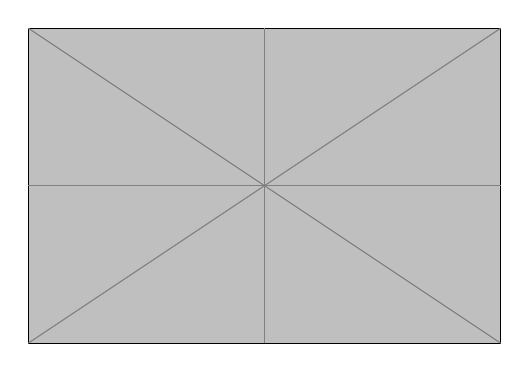
\begin{tikzpicture}
        \draw[black,fill=gray!50] (0,0) rectangle (6,4);
          \draw[gray,thin] (0,0) -- (6,4);
          \draw[gray,thin] (0,4) -- (6,0);
          \draw[gray,thin] (3,0) -- (3,4);
          \draw[gray,thin] (0,2) -- (6,2);
          \node at (3,2) {\tikz\randuck;};
      \end{tikzpicture}}
  }%<<<
%    \end{macrocode}
% \end{macro}^^A<<<
%^^A<<<
%
% \subsubsection{Intern}^^A>>>
%
% \begin{macro}{\duckuments@headings}^^A>>>
%    \begin{macrocode}
\newcommand*\duckuments@headings[1]
  {%>>>
    \ifcase#1\relax
      \expandafter\chapter
    \or \expandafter\section
    \or \expandafter\subsection
    \or \expandafter\subsubsection
    \or \expandafter\paragraph
    \else \expandafter\@gobble
    \fi
    {\duckuments@headings@text{#1}}
  }%<<<
%    \end{macrocode}
% \end{macro}^^A<<<
%
% \begin{macro}{\duckuments@headings@level}^^A>>>
%    \begin{macrocode}
\newcommand*\duckuments@headings@level[1]
  {%>>>
    (
    \ifcase#1
      chapter
    \or section
    \or subsection
    \or subsubsection
    \or paragraph
    \fi
    )
  }%<<<
%    \end{macrocode}
% \end{macro}^^A<<<
%
% \begin{macro}{\duckuments@ifinline}^^A>>>
%    \begin{macrocode}
\newcommand*\duckuments@ifinline[2][]
  { \bool_if:NTF \l_duckuments_math_inline_bool { #2 } { #1 } }
%    \end{macrocode}
% \end{macro}^^A<<<
%
% \begin{macro}{\duckuments@ifdisplay}^^A>>>
%    \begin{macrocode}
\newcommand*\duckuments@ifdisplay[2][]
  { \bool_if:NTF \l_duckuments_math_display_bool { #2 } { #1 } }
%    \end{macrocode}
% \end{macro}^^A<<<
%
% \begin{macro}{\duckuments_list_example:n}^^A>>>
%    \begin{macrocode}
\cs_new_protected_nopar:Nn \duckuments_list_example:n
  {%>>>
    \subsection{Example\ for\ ducks\ (#1)}
    \ducklist { #1 }
    \subsubsection{Nested\ ducks}
    \ducklistlist { #1 }
  }%<<<
%    \end{macrocode}
% \end{macro}^^A<<<
%
% \begin{macro}{\duckuments@enquote}^^A>>>
%    \begin{macrocode}
\newcommand*\duckuments@enquote [1]
  {%>>>
    \cs_if_exist_use:NTF
      \enquote { #1 }
      {``#1''}
  }%<<<
%    \end{macrocode}
% \end{macro}^^A<<<
%
% \begin{macro}{\duckuments_patch_includegraphics:}^^A>>>
%    \begin{macrocode}
\cs_new_protected_nopar:Nn \duckuments_patch_includegraphics:
  {%>>>
    \cs_if_exist:NT \includegraphics
      {
        \LetLtxMacro\duckuments@includegraphicsBAK\includegraphics
        \RenewDocumentCommand \includegraphics
          { >{\duckuments_starred:n}s O{} m }
          {
            \regex_match:NnTF \c_duckuments_example_regex { ##3 }
              {
                \duckuments_get_random_page:
                \duckuments@includegraphicsBAK##1
                  [page=\duckuments_random_page:,##2]
                  { ##3 }
              }
              {
                \duckuments@includegraphicsBAK##1[##2]{##3}
              }
          }
      }
  }%<<<
%    \end{macrocode}
% \end{macro}^^A<<<
%
% \begin{macro}{\duckuments_blindduck_range_test:n}^^A>>>
%    \begin{macrocode}
\cs_new_protected:Nn \duckuments_blindduck_range_test:n
  {%>>>
    \regex_match:NnTF \c_duckuments_range_regex { #1 }
      {
        \seq_set_split:Nnn \l_duckuments_range_seq { - } { #1 }
        \int_compare:nNnTF { 1 } = { \seq_count:N \l_duckuments_range_seq }
          {
            \cs_set:Npn \duckuments@blindduck@text
              {
                \duckuments_blindduck_single_par:n { #1 } 
                \int_gset:Nn \g_duckuments_blindduck_start_int { #1 + \c_one }
              }
          }
          {
            \bool_set_true:N \l_duckuments_blindduck_pars_bool
            \exp_args:Nx
            \tl_if_empty:nF { \seq_item:Nn \l_duckuments_range_seq { \c_one } }
              {
                \int_gset:Nn \g_duckuments_blindduck_start_int
                  { \seq_item:Nn \l_duckuments_range_seq { \c_one } }
              }
            \exp_args:Nx
            \tl_if_empty:nTF { \seq_item:Nn \l_duckuments_range_seq { \c_two } }
              {
                \int_gset_eq:NN
                  \g_duckuments_blindduck_end_int
                  \g_duckuments_blindduck_start_int
              }
              {
                \int_set:Nn \g_duckuments_blindduck_end_int
                  { \seq_item:Nn \l_duckuments_range_seq { \c_two } }
              }
            \duckuments_blindduck_set_text:xx
              { \int_use:N \g_duckuments_blindduck_start_int }
              { \int_use:N \g_duckuments_blindduck_end_int }
          }
      }
      {
        \group_begin:
          \exp_args:NnnV
            \msg_error:nnn { duckuments } { option~unknown } \l_keys_key_tl
        \group_end:
      }
  }%<<<
\cs_generate_variant:Nn \duckuments_blindduck_range_test:n { V }
%    \end{macrocode}
% \end{macro}^^A<<<
%
% \begin{macro}{\duckuments_blindduck_set_text:nn}^^A>>>
%    \begin{macrocode}
\cs_new:Nn \duckuments_blindduck_set_text:nn
  {%>>>
    \def \duckuments@blindduck@text
      {
        \int_step_function:nnnN { #1 } { \c_one } { #2 }
          \duckuments_blindduck_par_loop:n
        \int_gset:Nn \g_duckuments_blindduck_start_int { #2 + \c_one }
      }
  }%<<<
\cs_generate_variant:Nn \duckuments_blindduck_set_text:nn { xx }
%    \end{macrocode}
% \end{macro}^^A<<<
%
% \begin{macro}{\duckuments_blindduck_single_par:n}^^A>>>
%    \begin{macrocode}
\cs_new:Nn \duckuments_blindduck_single_par:n
  {%>>>
    \bool_if:nTF
      {
        \int_compare_p:nNn { #1 } > { \c_duckuments_blindduck_pars_int }
        || \int_compare_p:nNn { #1 } < { \c_one }
      }
      {
        \msg_error:nnxxxx { duckuments } { out~of~range }
          { 1 } { \int_use:N \c_duckuments_blindduck_pars_int } { #1 }
          { blindduck~paragraphs }
        \duckuments@blindduck@text@i
      }
      {
        \use:c { duckuments@blindduck@text@ \int_to_roman:n { #1 } }
      }
  }%<<<
%    \end{macrocode}
% \end{macro}^^A<<<
%
% \begin{macro}{\duckuments_blindduck_par_loop:n}^^A>>>
%    \begin{macrocode}
\cs_new:Nn \duckuments_blindduck_par_loop:n
  {%>>>
    \duckuments_blindduck_single_par:n { #1 }
    \par
  }%<<<
%    \end{macrocode}
% \end{macro}^^A<<<
%
% \begin{macro}{\duckuments_starred:n}^^A>>>
%    \begin{macrocode}
\cs_new_protected:Nn \duckuments_starred:n
  {%>>>
    \IfBooleanTF { #1 }
      { \def\ProcessedArgument{*} }
      { \def\ProcessedArgument{} } 
  }%<<<
%    \end{macrocode}
% \end{macro}^^A<<<
%
% \begin{macro}{\duckuments_get_random_page:, \duckuments_random_page:}^^A>>>
%    \begin{macrocode}
\sys_if_engine_xetex:TF
  {
%    \end{macrocode}
% For \XeTeX\ we need a bit more code in order to get random numbers. The
% following is an implementation of RC4. First declare some variables:
%    \begin{macrocode}
    \int_new:N \g_duckuments_RCiv_i_int
    \int_new:N \g_duckuments_RCiv_j_int
    \int_new:N \g_duckuments_RCiv_keylength_int
    \int_new:N \g_duckuments_tmpa_int
    \int_const:Nn \c_duckuments_RCiv_Slength_int { 256 }
    \tl_new:N \l_duckuments_tmpa_tl
    \tl_new:N \l_duckuments_tmpb_tl
%    \end{macrocode}
% Initialize the S array:
%    \begin{macrocode}
    \cs_new_protected_nopar:Nn \duckuments_RCiv_S_new:n
      { \int_new:c { g_duckuments_RCiv_S_ \int_eval:n { #1 } _int } }
    \cs_new_protected_nopar:Nn \duckuments_RCiv_S_set:nn
      { \int_gset:cn { g_duckuments_RCiv_S_ \int_eval:n { #1 } _int } { #2 } }
    \cs_new_nopar:Nn \duckuments_RCiv_S_get:n
      { \int_use:c { g_duckuments_RCiv_S_ \int_eval:n { #1 } _int } }
    \cs_new_protected_nopar:Nn \duckuments_RCiv_key_new:n
      { \int_new:c { g_duckuments_RCiv_key_ \int_eval:n { #1 } _int } }
    \cs_new_protected_nopar:Nn \duckuments_RCiv_key_set:nn
      { \int_gset:cn { g_duckuments_RCiv_key_ \int_eval:n { #1 } _int } { #2 } }
    \cs_new_nopar:Nn \duckuments_RCiv_key_get:n
      { \int_use:c { g_duckuments_RCiv_key_ \int_eval:n { #1 } _int } }
    \int_step_inline:nnnn { 0 } { 1 } { 255 }
      {
        \duckuments_RCiv_S_new:n { #1 }
        \duckuments_RCiv_S_set:nn { #1 } { #1 }
      }
    \int_step_inline:nnnn { 0 } { 1 } { 4 }
      { \duckuments_RCiv_key_new:n { #1 } }
    \duckuments_RCiv_key_set:nn { 0 } { \c_sys_minute_int }
    \duckuments_RCiv_key_set:nn { 1 } { \c_sys_hour_int }
    \duckuments_RCiv_key_set:nn { 2 } { \c_sys_day_int }
    \duckuments_RCiv_key_set:nn { 3 } { \c_sys_month_int }
    \duckuments_RCiv_key_set:nn { 4 }
      { \int_mod:nn { \c_sys_year_int } { \c_duckuments_RCiv_Slength_int } }
    \int_gset:Nn \g_duckuments_RCiv_keylength_int { 5 }
    \str_map_inline:Nn \c_sys_jobname_str
      {
        \duckuments_RCiv_key_new:n { \g_duckuments_RCiv_keylength_int }
        \duckuments_RCiv_key_set:nn
          { \g_duckuments_RCiv_keylength_int }
          { \int_from_alph:n { #1 } }
        \int_gincr:N \g_duckuments_RCiv_keylength_int
      }
    \cs_new_protected_nopar:Nn \duckuments_swap_S_entries:nn
      {
        \int_set_eq:Nc
          \g_duckuments_tmpa_int
          { g_duckuments_RCiv_S_ \int_eval:n { #1 } _int }
        \int_set_eq:cc
          { g_duckuments_RCiv_S_ \int_eval:n { #1 } _int }
          { g_duckuments_RCiv_S_ \int_eval:n { #2 } _int }
        \int_set_eq:cN
          { g_duckuments_RCiv_S_ \int_eval:n { #2 } _int }
          \g_duckuments_tmpa_int
      }
    \int_gset:Nn \g_duckuments_RCiv_keylength_int { 5 }
    \cs_new:Nn \duckuments_gadd_mod:Nnn
      { \int_gset:Nn #1 { \int_mod:nn { #1 + ( #2 ) } { #3 } } }
    \cs_new:Nn \duckuments_gadd_mod_Slength:Nn
      {
        \duckuments_gadd_mod:Nnn #1
          { #2 } { \c_duckuments_RCiv_Slength_int }
      }
    \int_step_inline:nnnn { 0 } { 1 } { 255 }
      {
        \int_gset:Nn \g_duckuments_tmpa_int
          { \int_mod:nn { #1 } { \g_duckuments_RCiv_keylength_int } }
        \duckuments_gadd_mod_Slength:Nn \g_duckuments_RCiv_j_int
          { 
            \duckuments_RCiv_S_get:n { #1 }
            + \duckuments_RCiv_key_get:n { \g_duckuments_tmpa_int }
          }
        \duckuments_swap_S_entries:nn { #1 } { \g_duckuments_RCiv_j_int }
      }
    \int_gzero:N \g_duckuments_RCiv_i_int
    \int_gzero:N \g_duckuments_RCiv_j_int
%    \end{macrocode}
% Provide a function which gets the next random number and sets
% |\duckuments_random_page:| to it.
%    \begin{macrocode}
    \cs_new_protected_nopar:Nn \duckuments_get_random_page:
      {
        \duckuments_gadd_mod_Slength:Nn \g_duckuments_RCiv_i_int { \c_one } 
        \duckuments_gadd_mod_Slength:Nn \g_duckuments_RCiv_j_int
          { \duckuments_RCiv_S_get:n { \g_duckuments_RCiv_i_int } }
        \duckuments_swap_S_entries:nn
          { \g_duckuments_RCiv_i_int }
          { \g_duckuments_RCiv_j_int }
        \int_gset:Nn \g_duckuments_tmpa_int
          { \duckuments_RCiv_S_get:n { \g_duckuments_RCiv_i_int } }
        \duckuments_gadd_mod_Slength:Nn \g_duckuments_tmpa_int
          { \duckuments_RCiv_S_get:n { \g_duckuments_RCiv_j_int } }
        \cs_set:Nx \duckuments_random_page:
          {
            \int_eval:n
              {
                \int_mod:nn
                  { \duckuments_RCiv_S_get:n { \g_duckuments_tmpa_int } }
                  { \c_duckuments_example_pages_int }
                + \c_one
              }
          }
      }
    \cs_new:Nn \duckuments_random_page: { 1 }
  }
%    \end{macrocode}
% Both \pdfTeX\ and \LuaTeX\ don't need the RC4 as there |\int_random:nn| is
% available.
%    \begin{macrocode}
  {
    \cs_new:Nn \duckuments_get_random_page: {}
    \cs_new:Nn \duckuments_random_page:
      { \int_rand:nn { 1 } { \c_duckuments_example_pages_int } }
  }
%    \end{macrocode}
% \end{macro}^^A<<<
%
%    \begin{macrocode}
\ExplSyntaxOff
%    \end{macrocode}
%
% \begin{macro}{\duckuments@blindduck@text}^^A>>>
%    \begin{macrocode}
\newcommand*\duckuments@blindduck@text{\duckuments@blindduck@text@i}
\newcommand*\duckuments@blindduck@text@i
  {%>>>
    There once was a very smart but sadly blind duck. When it was still a small
    duckling it was renowned for its good vision. But sadly as the duck grew
    older it caught a sickness which caused its eyesight to worsen. It became so
    bad, that the duck couldn't read the notes it once took containing much of
    inline math\duckuments@ifinline{ just like its favoured equation: $d = u_c
    \cdot k$}. Only displayed equations remained legible%
    \duckuments@ifdisplay[.]{ so it could still read \begin{equation}d = r a^k
    e\hbox{.}\end{equation}} That annoyed the smart duck, as it wasn't able to
    do its research any longer. It called for its underduckling and said:
    \duckuments@enquote{Go, find me the best eye ducktor there is. He shall
    heal me from my disease!}%
  }%<<<
\newcommand*\duckuments@blindduck@text@ii
  {%>>>
    \duckuments@enquote{But my duck, how are you supposed to manage your daily
    routines without my visual guidance}, replied the underduckling. The smart
    duck's face turned grim in anger. \duckuments@enquote{You dare to talk
    back?} The underduckling blushed ashamed. How could he have objections
    after his duck gave strict orders? The underduckling was so embarrassed
    about his own behaviour he had to solve an equation.%
  }%<<<
\newcommand*\duckuments@blindduck@text@iii
  {%>>>
    After the equation was solved and the underduckling prepared his leave for
    the next day it fell asleep in a shaky mood. It did not know what the
    journey had prepared for him and if he was prepared enough for it. His sleep
    was restless. The dreams he had that night were not calm and bright as they
    used to be for an innocent underduckling.%
  }%<<<
\newcommand*\duckuments@blindduck@text@iv
  {%>>>
    Before the first sunlight the underduckling woke. He didn't have the feeling
    of being well rested. But nonetheless he knew that this was the day he
    should leave. Except saying goodbye to his beloved ones there was nothing
    holding him back. His duck had sent him on the most important mission a five
    weeks old inexperienced underduckling was ever sent. He bid farewell to his
    mother, all his brothers and sisters, and finally from his duck. The bag was
    shouldered, the boots were tied, the underduckling left.%
  }%<<<
%    \end{macrocode}
% \end{macro}^^A<<<
%
% \begin{macro}{\duckuments@headings@text}^^A>>>
%    \begin{macrocode}
\newcommand*\duckuments@headings@text[1]
  {A friendly duck at level #1 \duckuments@headings@level{#1}}
%    \end{macrocode}
% \end{macro}^^A<<<
%
% \begin{macro}{\ducklists@content}^^A>>>
%    \begin{macrocode}
\newcommand*\ducklists@content
  {%>>>
    \item First swims father drake
    \item Then floats mother duck
    \item After her paddles baby duckling
    \item And over there bathes uncle canard
  }%<<<
%    \end{macrocode}
% \end{macro}^^A<<<
%
% \begin{macro}{\ducklists@content@starred}^^A>>>
%    \begin{macrocode}
\newcommand*\ducklists@content@starred
  {%>>>
    \item[drake] is the swimming father
    \item[duck] is the floating mother
    \item[duckling] is the paddling baby
    \item[canard] is the bathing uncle
  }%<<<
%    \end{macrocode}
% \end{macro}^^A<<<
%
% \begin{macro}{\duckuments@listlist}^^A>>>
%    \begin{macrocode}
\newcommand*\duckuments@listlist[1]
  {%>>>
    \begin{#1}
      \item swimming father drake
        \begin{#1}
          \item swimming father drake
            \begin{#1}
              \item swimming father drake
                \begin{#1}
                  \item swimming father drake
                  \item floating mother duck
                \end{#1}
              \item floating mother duck
            \end{#1}
          \item floating mother duck
        \end{#1}
      \item floating mother duck
    \end{#1}%
  }%<<<
%    \end{macrocode}
% \end{macro}^^A<<<
%
% \begin{macro}{\duckuments@listlist@starred}^^A>>>
%    \begin{macrocode}
\newcommand*\duckuments@listlist@starred[1]
  {%>>>
    \begin{#1}
      \item[drake] is the swimming father
        \begin{#1}
          \item[drake] is the swimming father
            \begin{#1}
              \item[drake] is the swimming father
                \begin{#1}
                  \item[drake] is the swimming father
                  \item[duck] is the floating mother
                \end{#1}
              \item[duck] is the floating mother
            \end{#1}
          \item[duck] is the floating mother
        \end{#1}
      \item[duck] is the floating mother
    \end{#1}%
  }%<<<
%    \end{macrocode}
% \end{macro}^^A<<<
%^^A<<<
%^^A<<<
%
%    \begin{macrocode}
\endinput
%    \end{macrocode}
%
% \end{implementation}^^A<<<
%
%    \begin{macrocode}
%</pkg>
%    \end{macrocode}
%
% \clearpage
% \section{The story of the duck}^^A>>>
%
% \blindduck[full]^^A<<<
%
^^A vim: fdm=marker foldmarker=>>>,<<<
